%%%%%%%%%%%%%%%%%%%%%%%%%%%%%%%%%%%%%%%%%%%%%%%%%%%%%
%				  Video In module					%
%					-----------						%
% Author: Vaibhav Singh	& Thibault Porteboeuf 		%
%%%%%%%%%%%%%%%%%%%%%%%%%%%%%%%%%%%%%%%%%%%%%%%%%%%%%

\section{Video-In module}
\begin{figure}[H]
\center
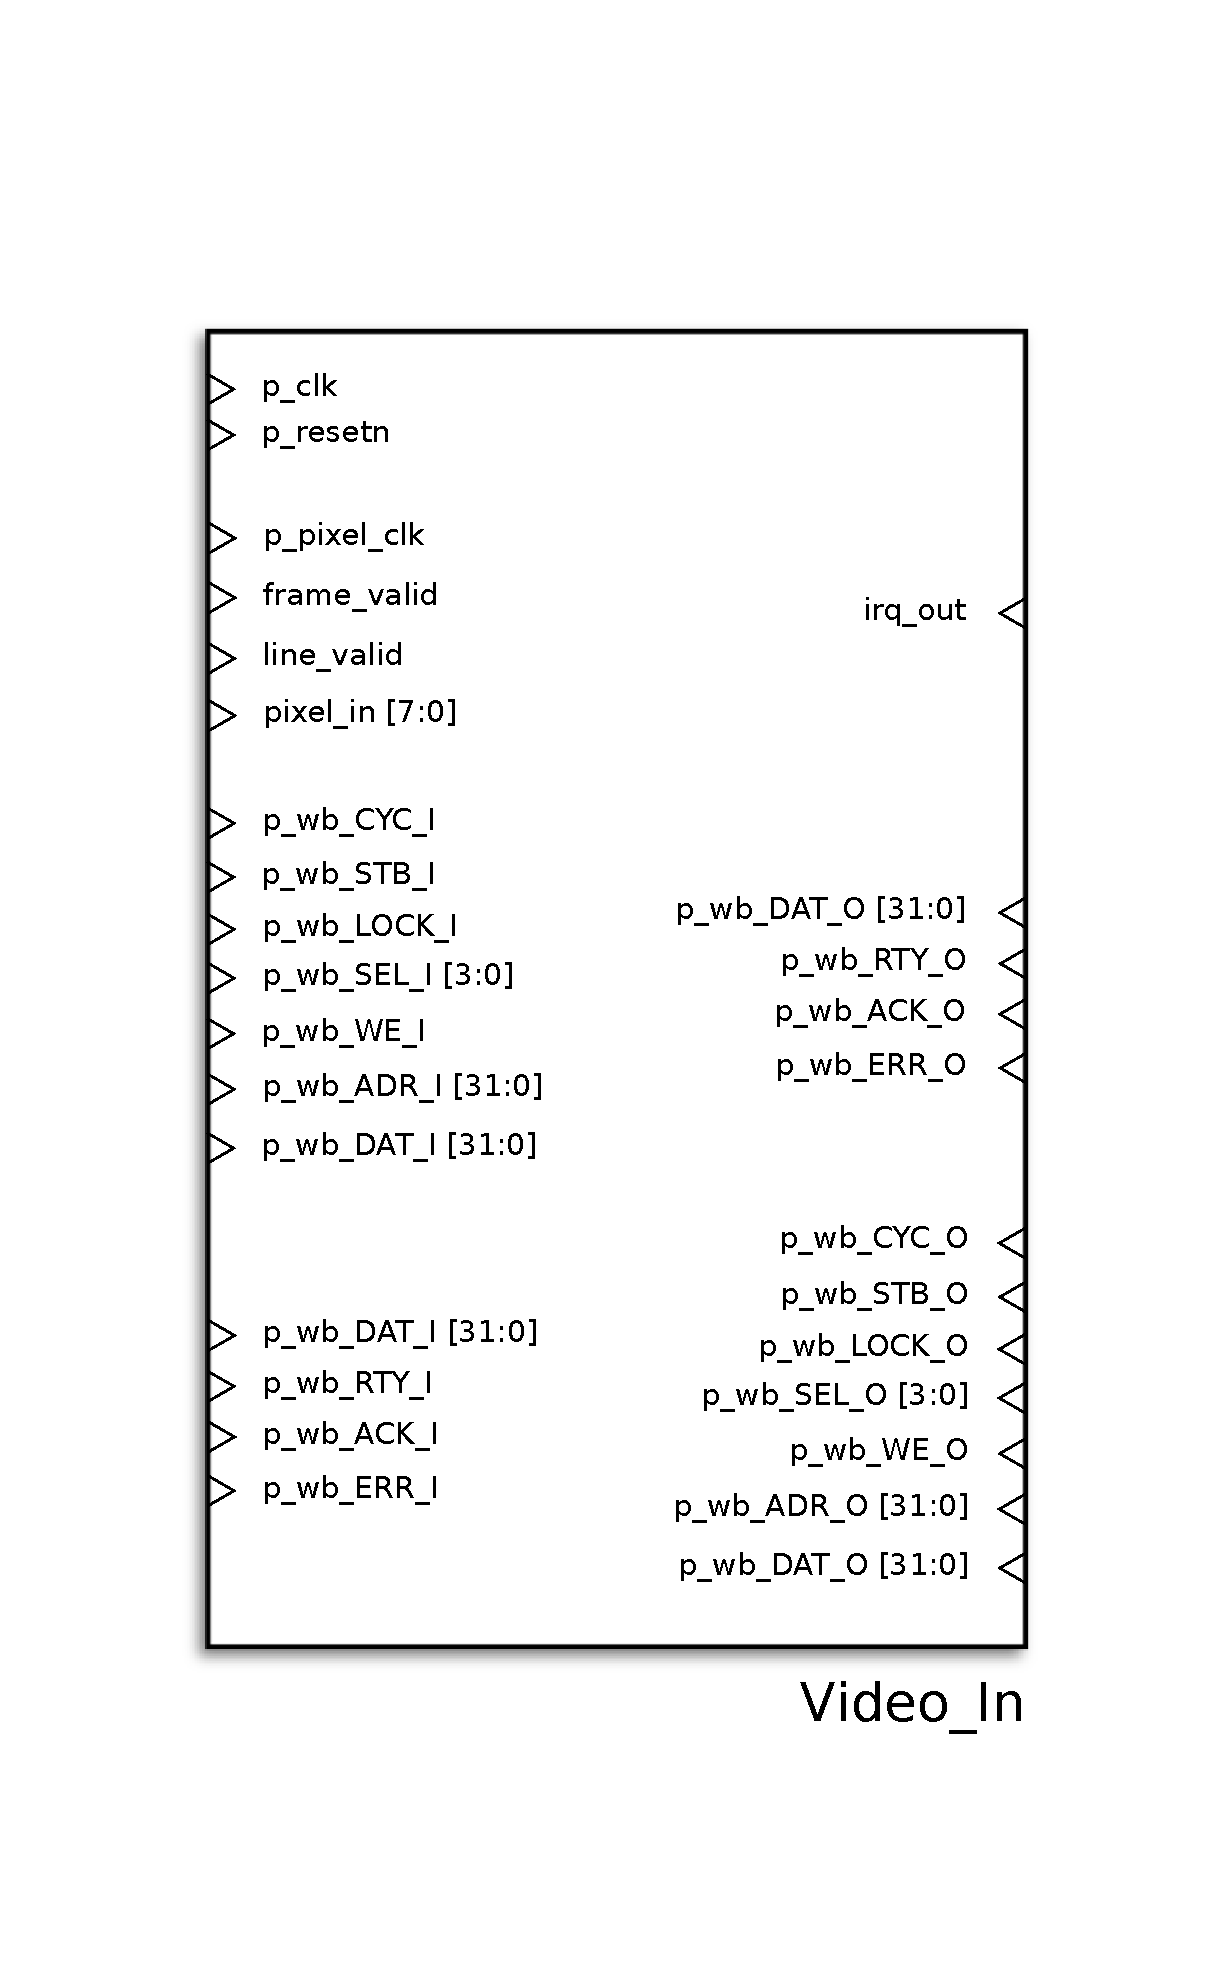
\includegraphics[width=7cm]{figs/Video_in.pdf}
\caption{Video-In module's interface}
\label{VideoIn_interface}
\end{figure}

As explained before, Video-In is the module responsible for handling the incoming video signals and transfer the pixels to the SRAM over the whishbone bus.

As described in the figure below, Video In Module has a Wishbone Master Module and another one which is a one register slave (as described in generic slave), as described in section \ref{wb_reg_slave}.

Video In has two blocks, one that takes pixels from video generator running at 25 Mhz, and other that stores data on to SRAM. Synchronisation of internal signals between the two different clock domains has been done.

The wishbone slave will handle incoming requests from the LM32, and store the content of write requests(start address of image) to its register. It is also responsible for driving the Irq(Interrupt Request) wire which will be raised to high whenver video in wants to request a new start address from LM32. The slave will automatically acknowledge when a write request is received.

The state machine samples the configuration stored in the slave's register at every rising edge of the \texttt{frame\_valid} signal. Thus, the configuration is updated only at the beginning of a new frame.

It then posts data from the buffer to the RAM, starting at the previously given address. This process is illustrated in figure \ref{VideoIn_sm}. 

Detailed explanation of video in can be found along the explanation of the source code.

\begin{figure}[h]
\center
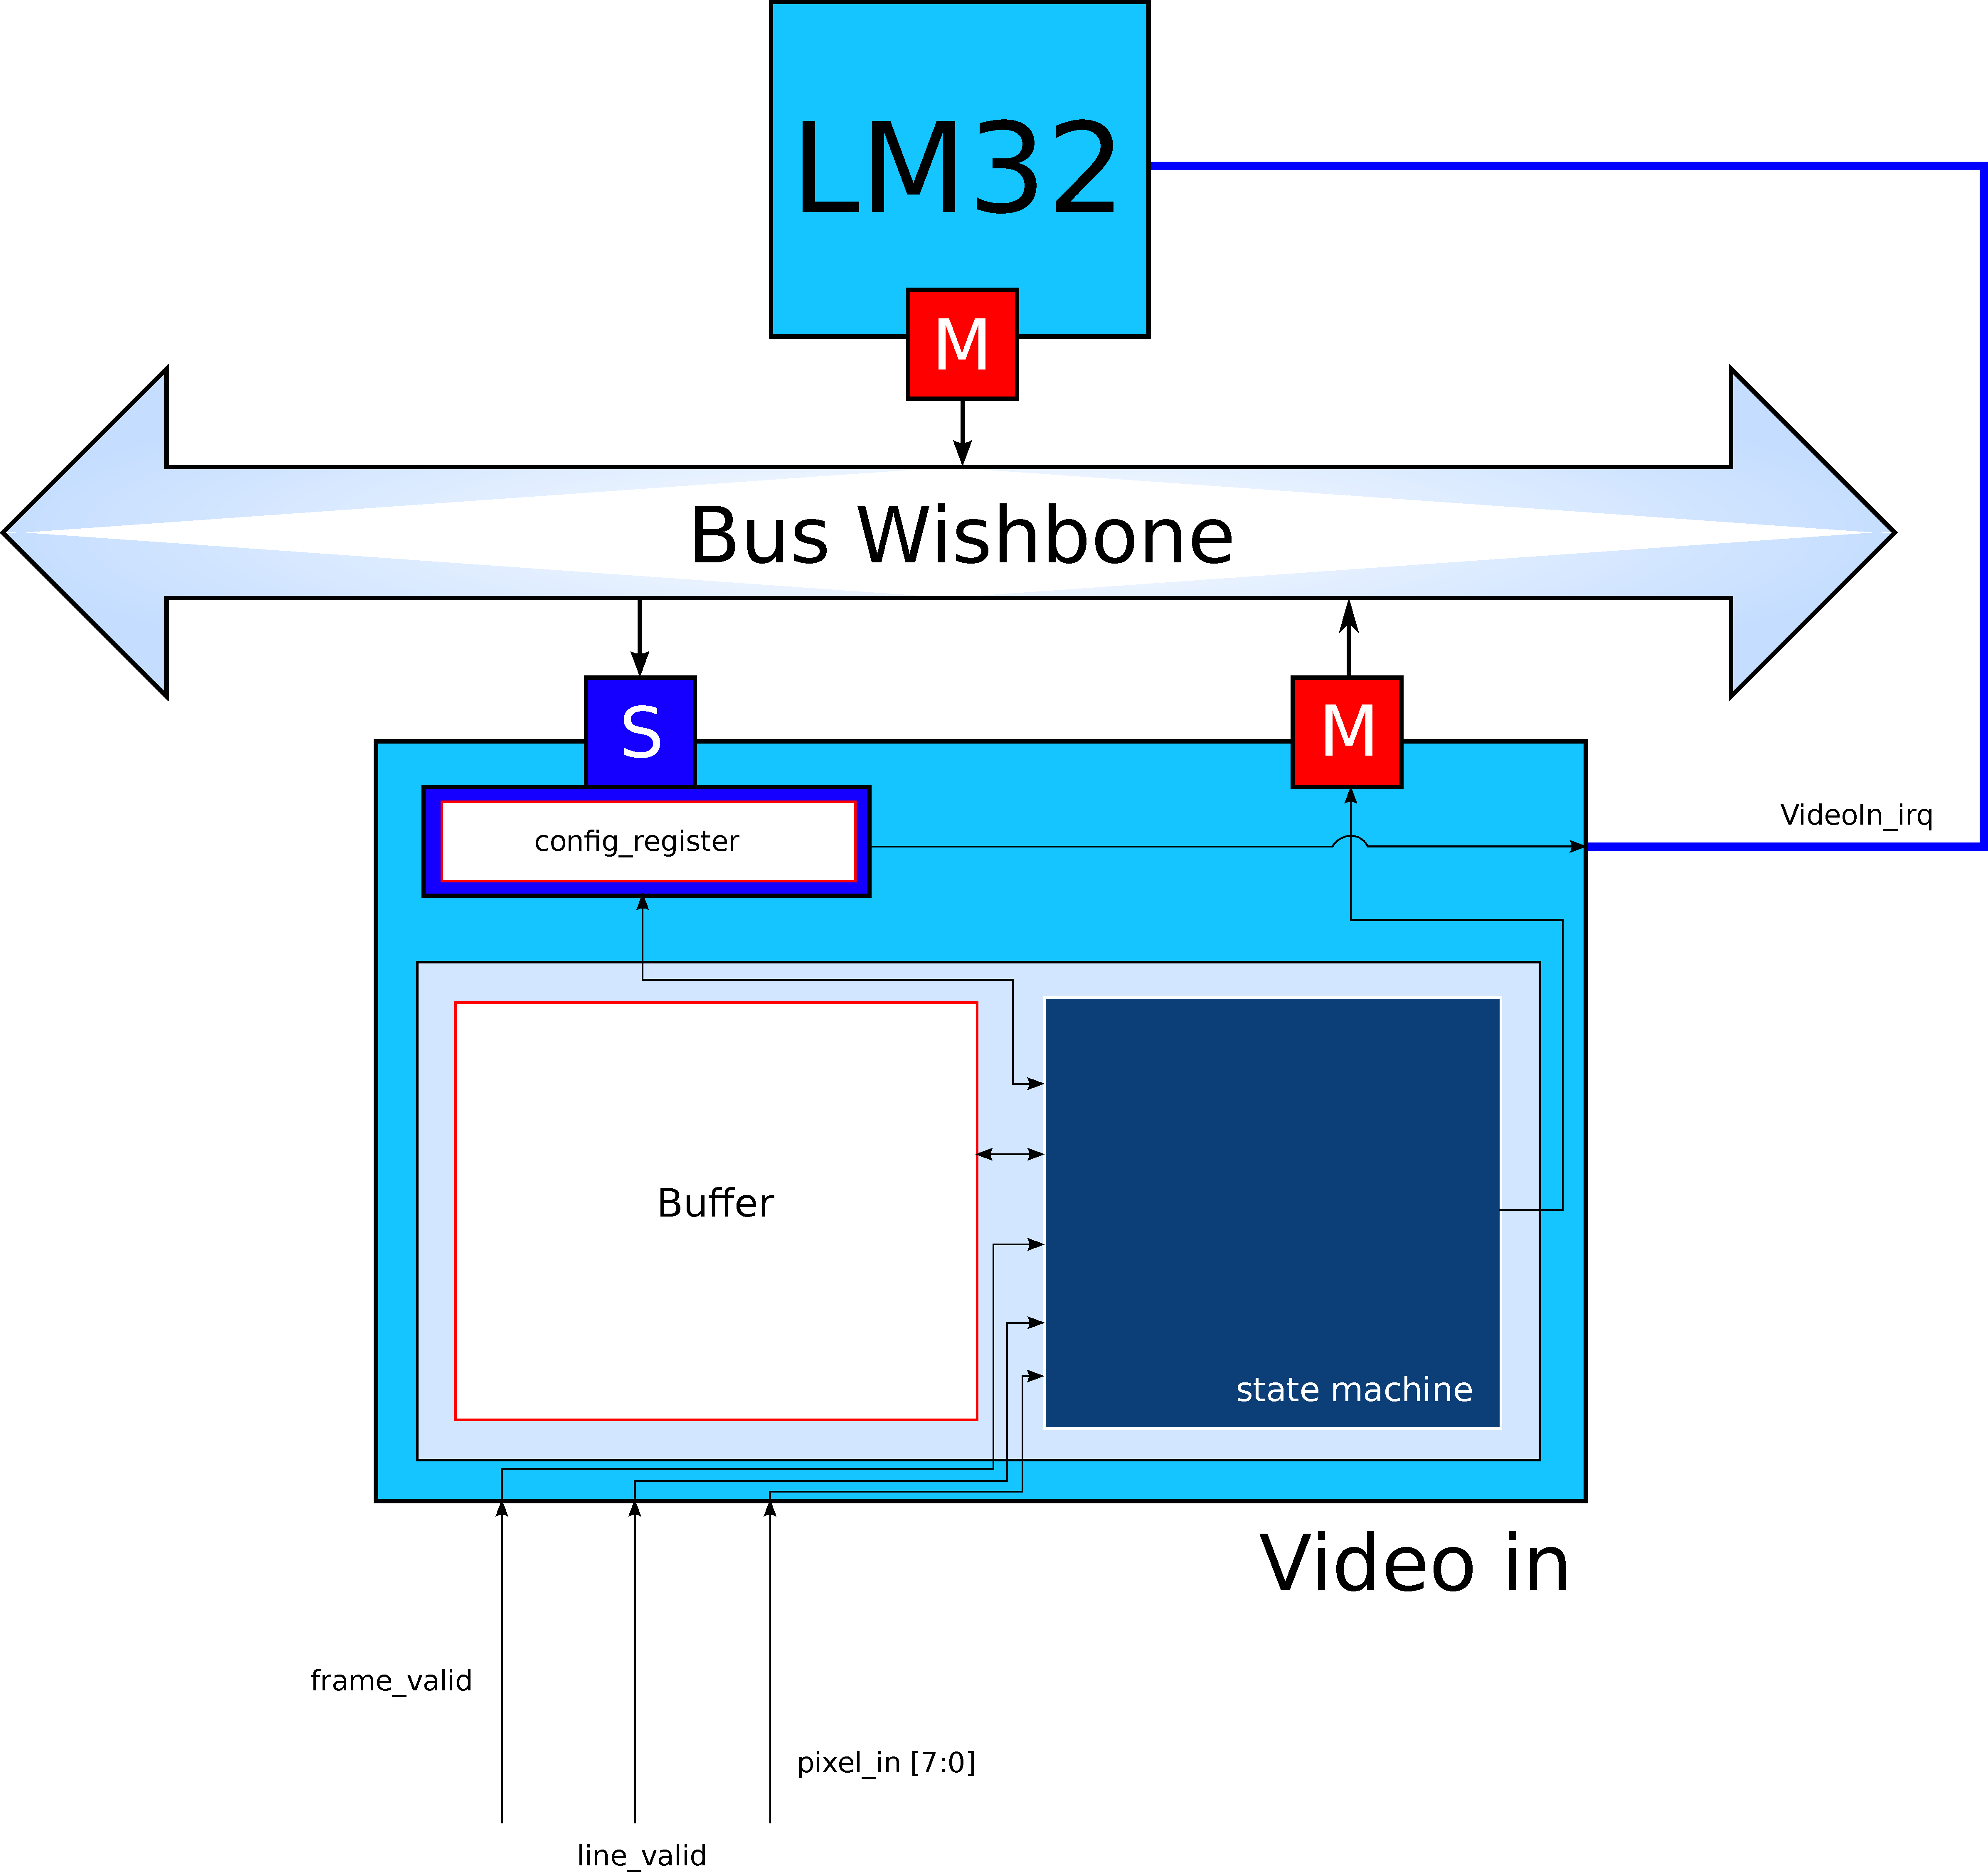
\includegraphics[width=11cm]{figs/Video_In_blocks.pdf}
\caption{VideoIn's inner structure}
\label{VideoIn_struct}
\end{figure}


\begin{figure}[h]
\center
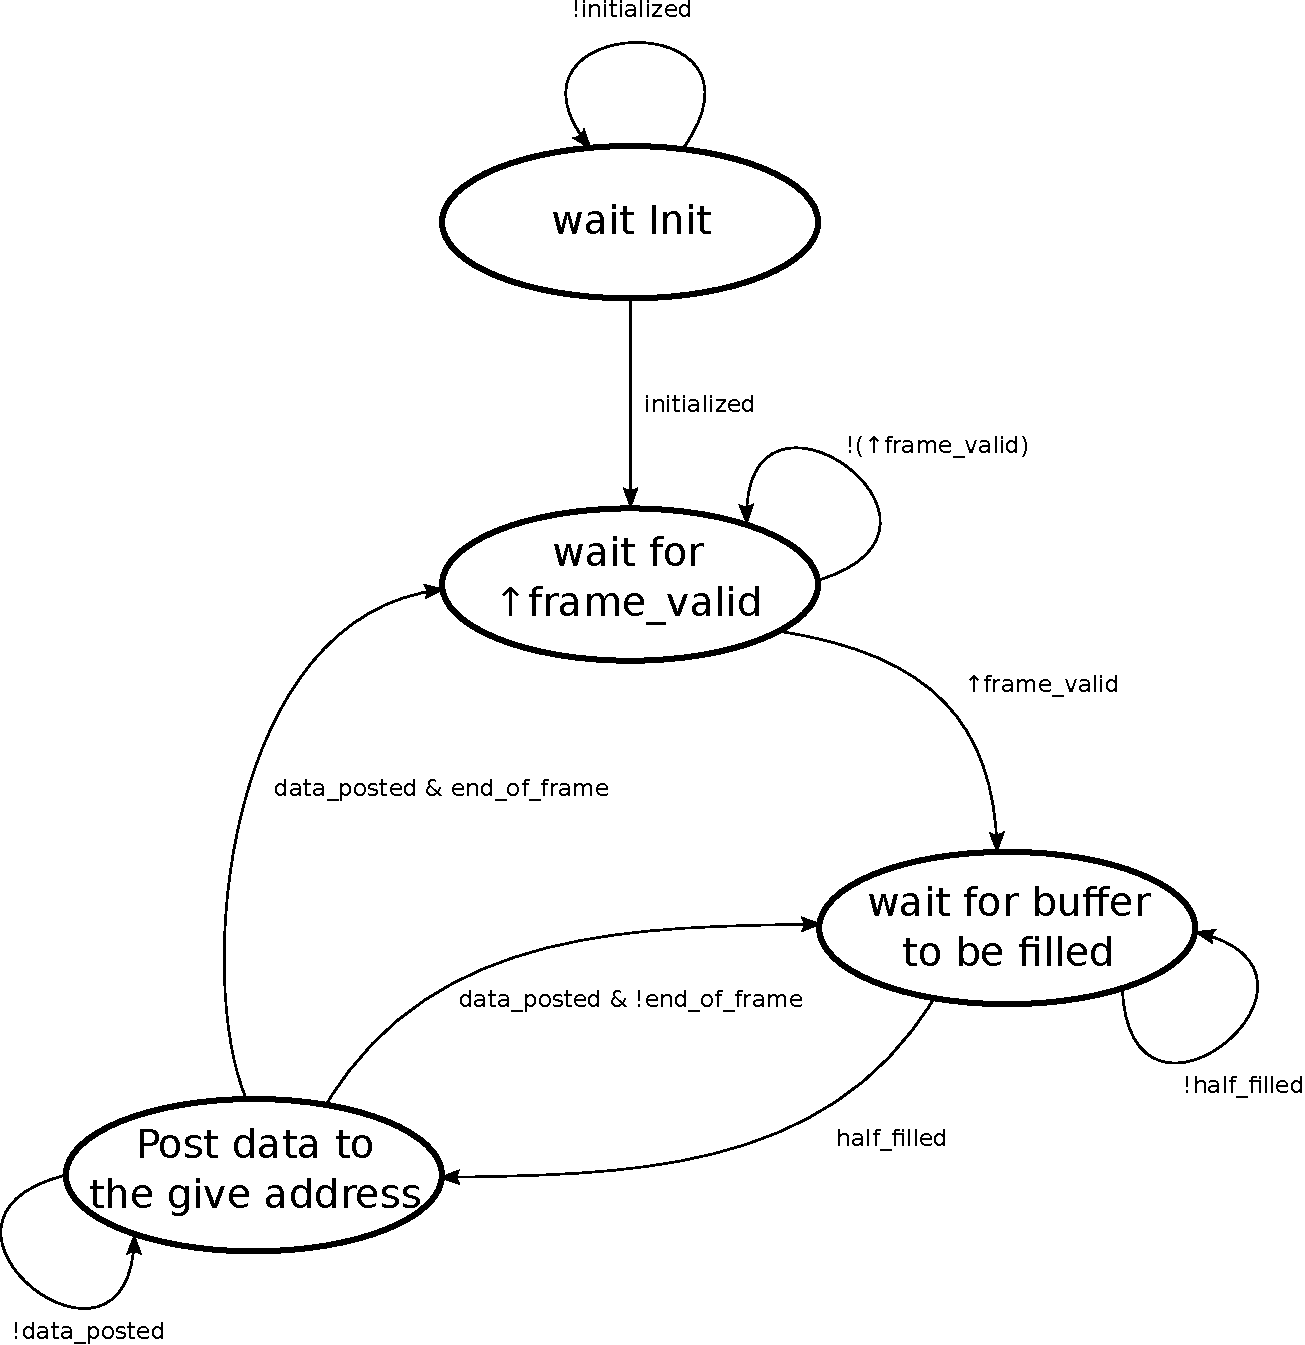
\includegraphics[width=11cm]{figs/video_in_sm.pdf}
\caption{VideoIn's behavior}
\label{VideoIn_sm}
\end{figure}

